\subsection{Attention forward pass}
\label{sec:fwd}



We first do a roofline analysis to show the bottlenecks of attention forward pass, which motivates our new pipeline design, as well as changes in the \fa algorithm to increase the throughput of the exponential unit and avoid most of the softmax rescaling steps.

\subsubsection{Feeds and Speeds}
\label{sec:fwd-feeds-and-speeds}

We provide intuition for our kernel design and optimizations by first analyzing the roofline, based on the throughput of the matmul units (tensor cores), shared memory (smem), and exponential unit. We note that this is a simplified analysis that does not consider all resources in the GPU (e.g., floating point math, register bandwidth, L2 bandwidth). Nevertheless, it can identify bottlenecks.

Let the shape of the tile along the length dimension of the sequence of $\vQ$ and $\vK$ be $M \times N$, and let the head dimension be $d$. We analyze the compute and memory traffic requirements to identify the performance bottleneck.

\noindent\textbf{MMA compute.}
The forward pass performs two matrix multiply-accumulate (MMA) operations per iteration: $\vQ\vK^\top$ (computing $M \times N$ output from $M \times d$ and $d \times N$ inputs) and $\vP\vV$ (computing $M \times d$ output from $M \times N$ and $N \times d$ inputs). Each MMA requires $2MNd$ floating-point operations. With a tensor core throughput of 8192 FLOPs per cycle, the total compute time is
{\setlength{\abovedisplayskip}{4pt}%
 \setlength{\belowdisplayskip}{4pt}%
 \setlength{\abovedisplayshortskip}{3pt}%
 \setlength{\belowdisplayshortskip}{3pt}%
\begin{equation}
    T_{\text{MMA}} = \frac{4MNd}{8192} \text{ cycles}.
\end{equation}}

\noindent\textbf{Shared memory traffic.}
Of the two MMAs, one is shared-shared (SS) where both operands are read from shared memory ($\vQ\vK^\top$), while the other is tensor-shared (TS) where operand $A$ is read from tensor memory and operand $B$ from shared memory ($\vP\vV$). Since each MMA instruction operates on tiles of size $128 \times 128$, computing an $M \times N$ output requires $\lceil M/128 \rceil \times \lceil N/128 \rceil$ MMA instructions. Crucially, when multiple MMA instructions are needed, the shared memory operands are read multiple times.

For $\vQ\vK^\top$ (SS), computing the $M \times N$ output requires $\lceil M/128 \rceil \times \lceil N/128 \rceil$ MMA instructions, each reading a $128 \times d$ chunk of $\vQ$ and a $d \times 128$ chunk of $\vK^\top$ from shared memory. The total shared memory reads are $\lceil M/128 \rceil \times \lceil N/128 \rceil \times (128d + 128d) = \lceil M/128 \rceil \lceil N/128 \rceil \times 256d$ elements. For $\vP\vV$ (TS), computing the $M \times d$ output requires $\lceil M/128 \rceil \times \lceil d/128 \rceil$ MMA instructions, each reading a $N \times 128$ chunk of $\vV$ from shared memory, totaling $\lceil M/128 \rceil \times \lceil d/128 \rceil \times 128N$ elements. At 2 bytes per element (bf16) and 128 bytes per cycle bandwidth, the shared memory ($T_{\text{smem}}$) read time is
{\setlength{\abovedisplayskip}{1pt}%
 \setlength{\belowdisplayskip}{0.1pt}%
 \setlength{\abovedisplayshortskip}{1pt}%
 \setlength{\belowdisplayshortskip}{0.1pt}%
\begin{equation}
  = 
  2\Big\lceil\tfrac{M}{128}\Big\rceil\Big\lceil\tfrac{N}{128}\Big\rceil 256d
+ 2\Big\lceil\tfrac{M}{128}\Big\rceil\Big\lceil\tfrac{d}{128}\Big\rceil 128N
= \tfrac{3MNd}{8192}\ \text{cycles}
\end{equation}}
(assuming $M$, $N$, $d$ are multiples of 128).

\noindent\textbf{Exponential unit.}
The exponential unit computes elementwise operations required for the softmax computation. The forward pass requires exponential operations on $M \times N$ values (corresponding to the attention matrix $\vS$). With a throughput of 16 operations per cycle, the exponential unit requires
{\setlength{\abovedisplayskip}{0.1pt}%
 \setlength{\belowdisplayskip}{1pt}%
 \setlength{\abovedisplayshortskip}{0.1pt}%
 \setlength{\belowdisplayshortskip}{1pt}%
\begin{equation}
    T_{\text{exp}} = \frac{MN}{16} \text{ cycles}.
\end{equation}}

Table~\ref{tab:fwd_roofline} summarizes the analysis for two typical tile configurations. For $M = N = d = 128$, the resources are well-balanced, with shared memory (768 cycles) being slightly lower than both MMA compute and exponential unit (both 1024 cycles). For the larger tile size $M = 256, N = d = 128$, the shared memory traffic increases to 1536 cycles due to reading MMA operands multiple times, while MMA compute and exponential unit double to 2048 cycles. This analysis motivates our kernel design to (1) use large tile sizes and maximize overlap between MMA operations and softmax computations (2) increase the throughput of exponential by using other hardware units (3) reduce the time of unnecessary non-matmul operations.

\begin{figure*}[t]
  \centering
  %\hspace*{0cm}
  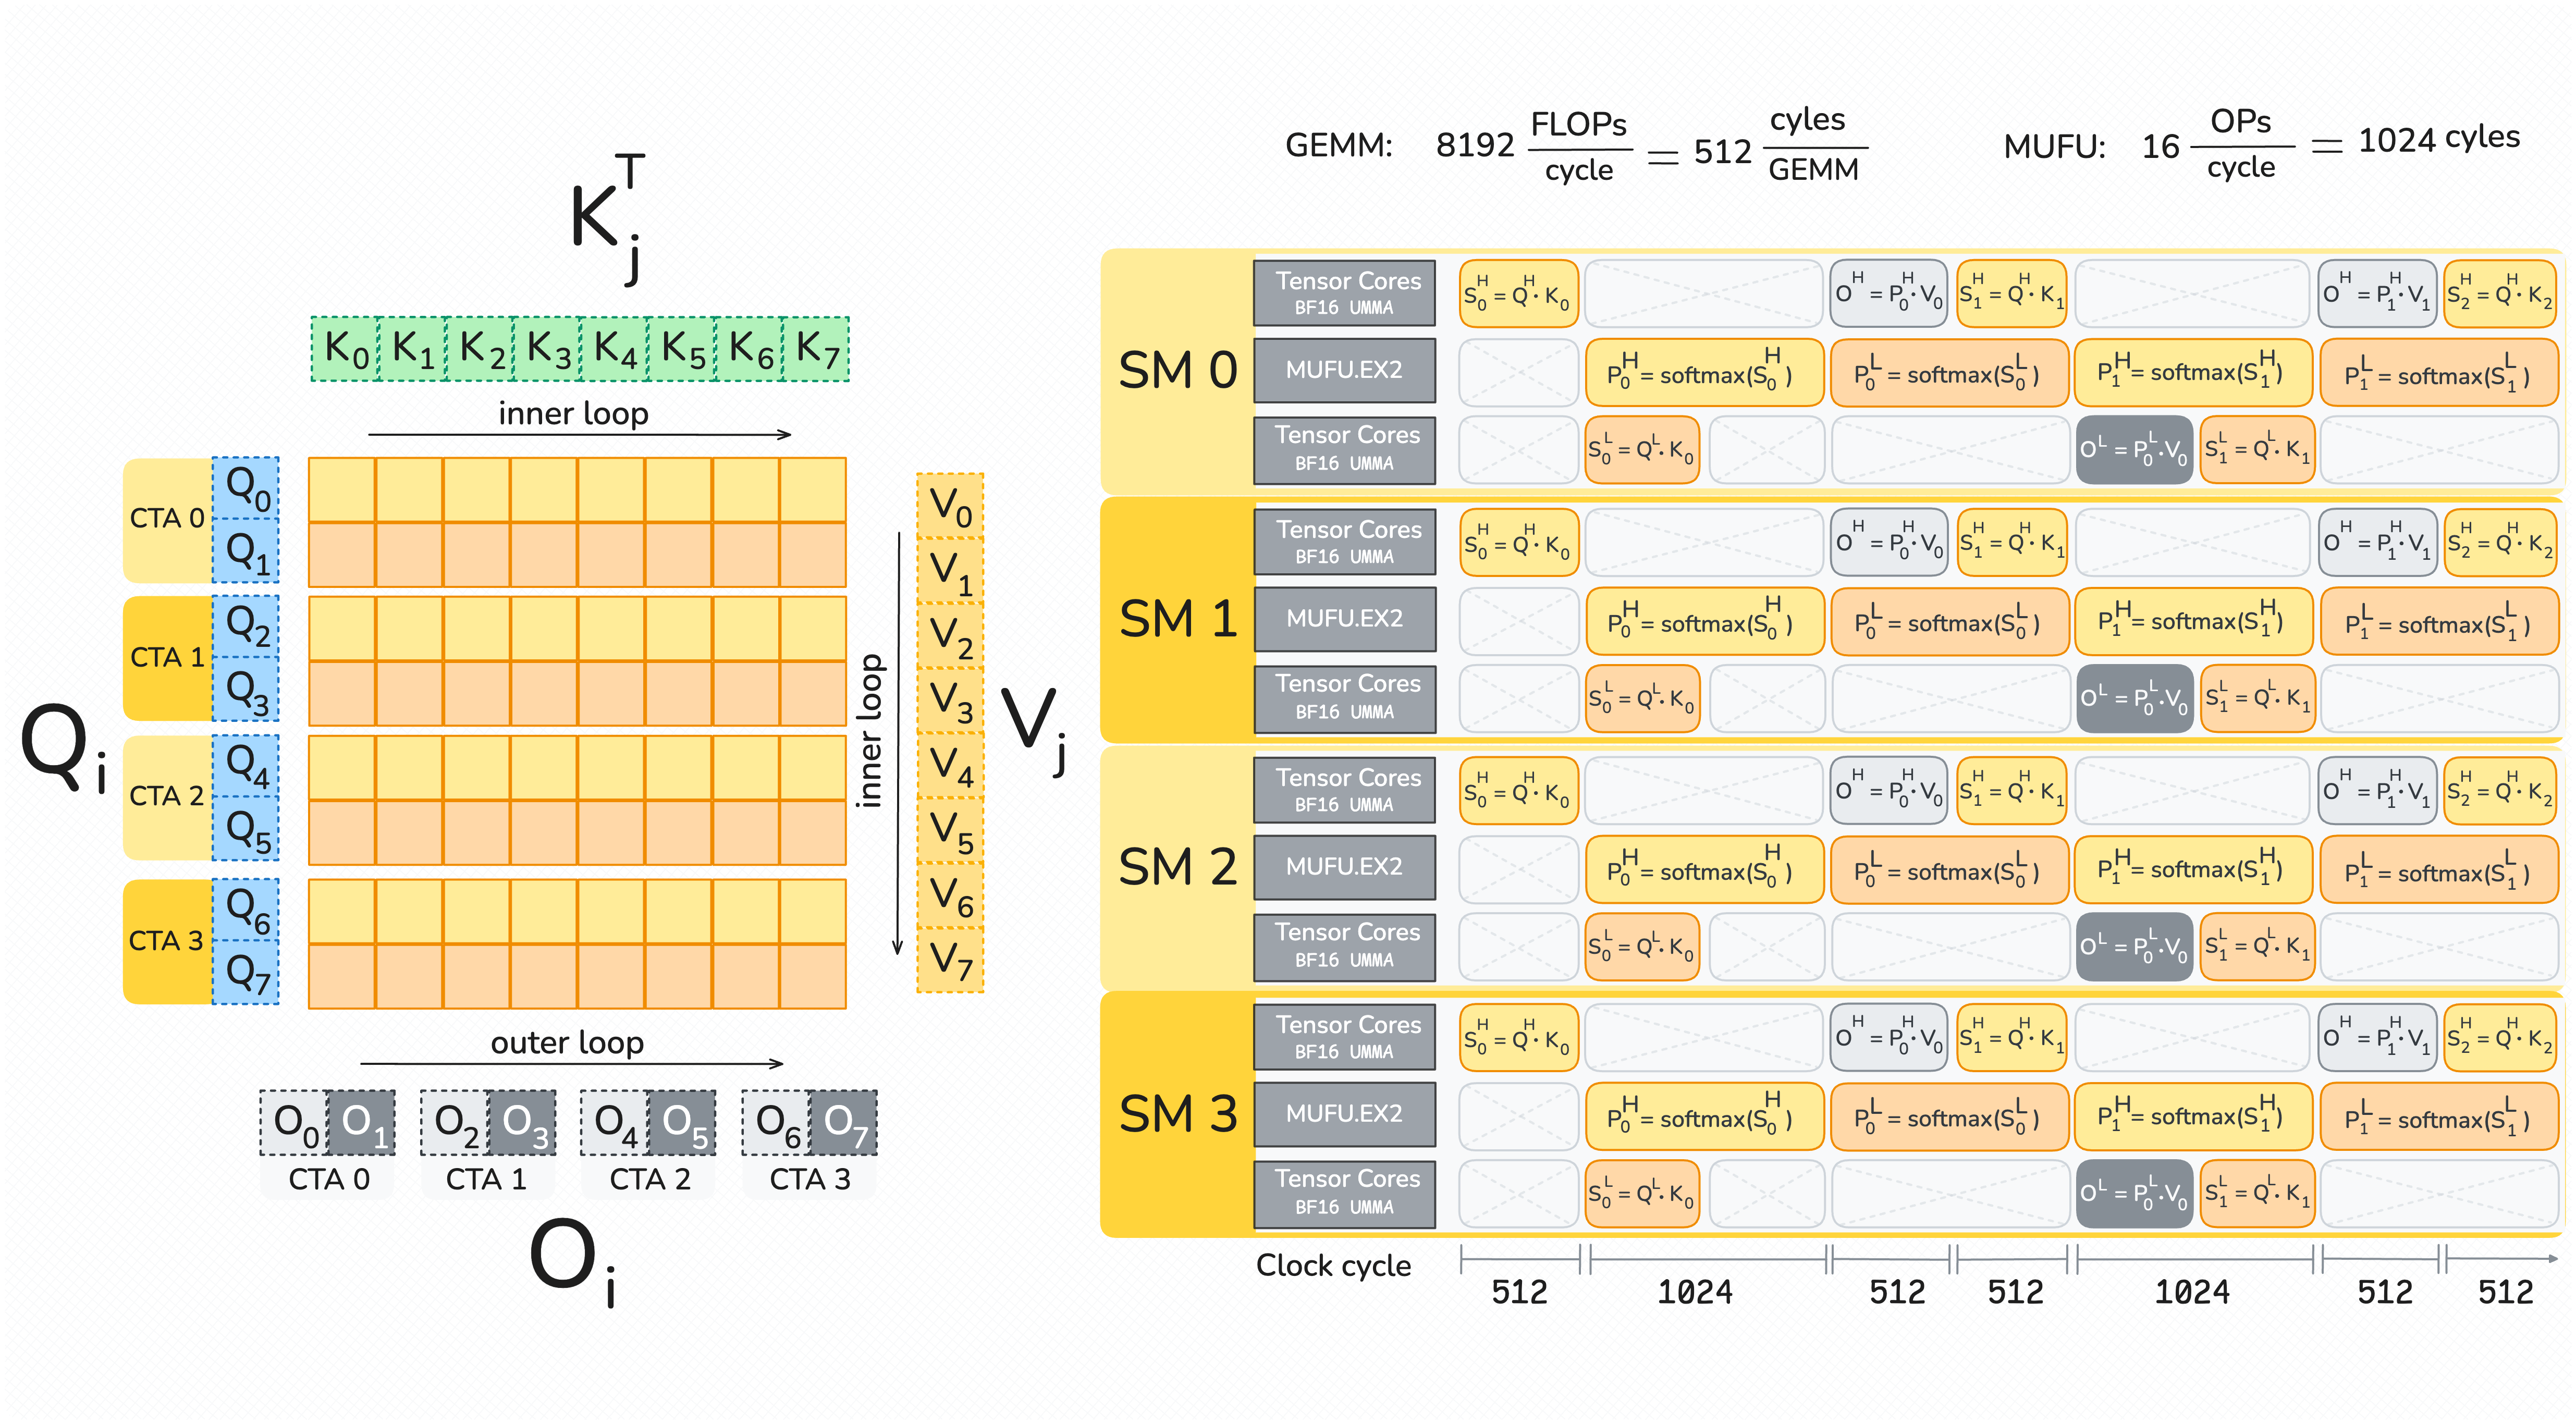
\includegraphics[width=1.0\linewidth]{../Figures/FA4_FWD_p3.png}
  \caption{FlashAttention-4 forward pipeline. The superscript $^H$ denotes the matrices corresponding to the "high" Q tile, and superscript $^L$ denotes matrices corresponding to the "low" Q tile. Each Q tile corresponds to 128 query tokens.}
  \label{fig:fwd_pipeline_wide}
\end{figure*}





\begin{table}[t]
\centering
\small
\begin{tabular}{lcc}
\toprule
Resource & $128^3$ & $256 \times 128^2$ \\
\midrule
MMA compute & \textbf{1024} & \textbf{2048} \\
Shared memory & 768 & 1536 \\
Exponential unit & \textbf{1024} & \textbf{2048} \\
\bottomrule
\end{tabular}
\caption{Roofline analysis (cycles) for the attention forward pass. For both tile sizes, MMA compute and exponential unit are the primary bottlenecks.}
\label{tab:fwd_roofline}
\end{table}

\subsubsection{New pipeline to overlap matmul and softmax}

Since the Blackwell architecture doubled the tensor core flops again, taking care to overlap softmax and tensor core operations is even more crucial than on Hopper. We follow a ping-pong schedule similar to FA-3, where two tiles of the output are computed per thread block.
While one tile's tensor core operations are executed, the other tile computes softmax.
While Hopper tensor cores hold the accumulator in registers, with four threads per row in an interleaved pattern, Blackwell tensor cores hold their accumulators in tensor memory.
Additionally, a single accumulator tile on Blackwell is 128 by 128 elements large, where Hopper's tile size was 64 by 128.

The natural way to distribute work across these tiles is then to have two warpgroups of 128 threads each, with each thread processing an entire row.
This eliminates the need for inter-warp shuffles to reduce the row max, and for multiple statistics registers per thread.
Just like with FA-3, we explicitly synchronize the two softmax warpgroups to not overlap in their critical section, which is the part of exponential computation.
Each softmax warpgroup proceeds by first loading the entire row into registers, then computing the maximum, then computing the softmax (i.e., subtract the max, rescale, exponentiate, convert to input precision), and finally computing the row sum.

Another difference from FA-3 is that since we transfer $\vP$ via tensor memory rather than register file, we can decouple the rescaling of the output to a separate ``correction'' warpgroup and thus take it out of the critical path.

Several tensor memory partitionings are possible to achieve this pipeline overlap. All must allocate two tiles worth of output, leaving (at head dimension 128) half the tensor memory to store $\vS$ and $\vP$. That memory can store two copies of $\vS$ or four copies of $\vP$ (assuming the input of the FP16 or BF16 tensor core).
This leaves us with roughly two partitioning options for the remaining tensor memory: one tile of $\vS$ and two tiles of $\vP$, or two tiles of $\vS$ that overlap with $\vP$. We choose the latter because it allows us to start our software pipeline by immediately computing two $\vS$ tiles. It also leaves some tensor memory to communicate rescale statistics to the correction warpgroup.

One issue of the larger Blackwell tile sizes and the chosen thread assignment is that, unless we re-load from tensor memory, we must hold an entire row of 128 elements in register.
Given that we use two softmax warpgroups, one correction warpgroup, and one warpgroup to drive tensor cores and TMA units, assigning sufficient registers to softmax and preventing register spills is critical.
For BF16 input data types, we need to hold 128 registers for the input, and potentially 64 registers for the output (plus miscellaneous and temporary registers).
To reduce register pressure, we stage out storing $\vP$: The first three quarters are stored once (and trigger the corresponding MMA operations), and the last quarter is stored separately.

\subsubsection{Emulation of the exponential function}

\textbf{Exponential throughput bottleneck.}
On modern GPUs, the exponential function is computed by the multi-function unit (MUFU), which has significantly lower throughput than the tensor cores used for matrix multiplication. On B200 and GB200 GPUs, MUFU provides 16 operations per clock per SM, compared to 8192 operations per clock per SM for matrix multiplication. Since softmax computation requires many exponential evaluations, this disparity makes the exponential function a critical bottleneck in attention kernels.

\textbf{Software emulation via polynomial approximation.}
To increase exponential throughput, we implement a software emulation of $2^x$ using floating-point FMA units, which can operate in parallel with MUFU. We use the classical range reduction technique (Cody-Waite) and then the polynomial approximation~\citep{muller2018handbook}. The key insight is to decompose the exponential computation:
{\setlength{\abovedisplayskip}{2pt}%
 \setlength{\belowdisplayskip}{2pt}%
 \setlength{\abovedisplayshortskip}{3pt}%
 \setlength{\belowdisplayshortskip}{3pt}%
\begin{equation}
2^x = 2^{\lfloor x \rfloor}\,2^{x-\lfloor x \rfloor}
\end{equation}}
where $\lfloor x \rfloor$ is the integer part and $x - \lfloor x \rfloor \in [0, 1)$ is the fractional part.

The integer part $2^{\lfloor x \rfloor}$ can be computed efficiently using bit manipulation of the IEEE 754 floating-point representation. Since the exponent field directly represents powers of two, computing $2^{\lfloor x \rfloor}$ amounts to a shift and add operation on the exponent bits, which can be done using integer ALU instructions.

For the fractional part, we approximate $2^{x_{\text{frac}}}$ where $x_{\text{frac}} \in [0, 1)$ using a polynomial:
\begin{equation}
2^{x_{\text{frac}}} \approx \sum_{i=0}^{n} p_i\, x_{\text{frac}}^i
\end{equation}
with $p_0 = 1.0$ and the remaining coefficients chosen to minimize the relative approximation error over $[0, 1)$, calculated using the Sollya software package~\citep{chevillard2010sollya}. The polynomial evaluation uses Horner's method with FMA instructions, achieving high throughput.

The complete algorithm proceeds as follows:
\begin{enumerate}
\item Clamp $x$ to be at least $-127$ to avoid underflow
\item Compute $\lfloor x \rfloor$ using round-down mode: add $2^{23} + 2^{22}$ to $x$ (forcing the fractional bits into the mantissa), then subtract it back with round-down mode
\item Compute fractional part: $x_{\text{frac}} = x - \lfloor x \rfloor$
\item Evaluate polynomial to get $2^{x_{\text{frac}}}$
\item Combine integer and fractional parts: shift $\lfloor x \rfloor$ into the exponent field and add the mantissa bits of $2^{x_{\text{frac}}}$
\end{enumerate}

By distributing exponential computations across both MUFU and FMA units, this approach effectively increases the exponential throughput, alleviating a key bottleneck in attention computation.

\textbf{Partial emulation.}
Although polynomial emulation increases exponential throughput, it comes at a cost: additional registers (to hold intermediate values and coefficients), higher register bandwidth consumption, and longer latency compared to the MUFU instruction. Using emulation for all exponential evaluations would increase register pressure and could cause spills that negate the throughput benefit. Instead, we apply emulation to only a subset of the entries in each softmax row (10--25\%), with the remaining entries computed via hardware \texttt{MUFU.EX2}. The exact fraction is tuned empirically based on the ratio of MMA and exponential throughput for a given tile configuration.

\textbf{Numerical accuracy.}
Table~\ref{tab:ex2_accuracy} compares the accuracy of polynomial approximations of different degrees against the hardware \texttt{MUFU.EX2} instruction, measured on 4M random inputs in $[0, 1)$. We report two metrics: the FP32-level error (before any quantization) and the BF16-level error (after rounding the FP32 output to BF16), both measured against a FP64 reference.

At the FP32 level, the degree-3 polynomial has a maximum relative error of $8.8 \times 10^{-5}$, roughly $600\times$ higher than hardware. However, after rounding to BF16, the errors become nearly indistinguishable: the quantization error of BF16 (${\sim}3.9 \times 10^{-3}$) dominates the polynomial approximation error for all degrees $\geq 3$. The degree-3 polynomial matches hardware to within 1~BF16 ~ ULP on 99\% of inputs, which is sufficient for attention computation where the softmax output is consumed with BF16 precision.
Higher-degree polynomials close the FP32 gap: degree~5 matches hardware to within $2\times$ in maximum relative error, at the cost of two additional FMA instructions per evaluation.

\begin{table}[t]
\centering
\small
\begin{tabular}{lccccc}
\toprule
& \multicolumn{2}{c}{FP32 vs FP64} & \multicolumn{2}{c}{BF16 vs FP64} \\
\cmidrule(lr){2-3} \cmidrule(lr){4-5}
Method & Max rel err & Mean rel err & Max rel err & Mean rel err \\
\midrule
Ideal (FP64$\to$BF16) & --- & --- & $3.89 \times 10^{-3}$ & $1.41 \times 10^{-3}$ \\
Hardware \texttt{MUFU.EX2} & $1.41 \times 10^{-7}$ & $3.04 \times 10^{-8}$ & $3.89 \times 10^{-3}$ & $1.41 \times 10^{-3}$ \\
Degree 3 & $8.77 \times 10^{-5}$ & $5.43 \times 10^{-5}$ & $3.90 \times 10^{-3}$ & $1.41 \times 10^{-3}$ \\
Degree 4 & $3.05 \times 10^{-6}$ & $1.84 \times 10^{-6}$ & $3.89 \times 10^{-3}$ & $1.41 \times 10^{-3}$ \\
Degree 5 & $1.44 \times 10^{-7}$ & $5.48 \times 10^{-8}$ & $3.89 \times 10^{-3}$ & $1.41 \times 10^{-3}$ \\
\bottomrule
\end{tabular}
\caption{Accuracy of $2^x$ polynomial emulation on $[0, 1)$, measured against FP64 reference on 4M random inputs. FP32 columns measure the raw polynomial output; BF16 columns measure after rounding to BF16. The BF16 quantization error dominates for all degrees $\geq 3$.}
\label{tab:ex2_accuracy}
\end{table}


\subsubsection{Skipping online softmax rescaling}

\textbf{FlashAttention online softmax.}
FlashAttention computes attention $\softmax(QK^\top)V$ in blocks to minimize memory traffic. For numerical stability, the algorithm maintains running statistics as it processes blocks. When computing block $j$, let $S_j = Q K_j^\top$ be the attention scores for that block. The online softmax algorithm tracks:
\begin{align*}
m_j &= \max(m_{j-1}, \rowmax(S_j)) \\
\ell_j &= e^{m_{j-1} - m_j} \ell_{j-1} + \rowsum(e^{S_j - m_j})
\end{align*}
where $m_j$ is the running max and $\ell_j$ is the running sum of exponentials (normalizer). The intermediate output $O_j$ is updated as:
$
O_j = e^{m_{j-1} - m_j} O_{j-1} + e^{S_j - m_j} V_j.
$
The rescaling factor $e^{m_{j-1} - m_j}$ ensures numerical stability by renormalizing previous results when larger values are encountered.

\textbf{Conditional rescaling.}
The step $e^{m_{j-1} - m_j} O_{j-1}$ requires a vector multiplication. We make two simple observations:
\begin{enumerate}
\item Rescaling is only necessary when $m_j > m_{j-1}$, i.e., when new larger values are found.
\item We can tolerate some "slack" in the rescaling: only rescale when $m_j - m_{j-1} > \tau$, where $\tau$ is a threshold (typically set to $\log_2(256) = 8.0$, corresponding to a rescaling factor of 256.0). As long as we keep track of the statistics (the total scaling we have done), we can still get the true denominator at the end to get the right final output. 
\end{enumerate}

In \faf, we modify the algorithm as:
\begin{equation}
O_j = \begin{cases}
e^{m_{j-1} - m_j} O_{j-1} + e^{S_j - m_j} V_j & \text{if } m_j - m_{j-1} > \tau \\
O_{j-1} + e^{S_j - m_{j-1}} V_j & \text{otherwise}
\end{cases}
\end{equation}
When $m_j - m_{j-1} \leq \tau$, we skip updating $m$ and continue using $m_{j-1}$. This maintains the correctness because at the end of the computation, all accumulated values are renormalized by the true maximum $m_{\text{final}}$ and the final normalizer $\ell_{\text{final}}$:
{\setlength{\abovedisplayskip}{0.1pt}%
 \setlength{\belowdisplayskip}{1pt}%
 \setlength{\abovedisplayshortskip}{0.1pt}%
 \setlength{\belowdisplayshortskip}{1pt}%
\begin{equation*}
\text{Output} = \frac{1}{\ell_{\text{final}}} O_{\text{final}}
\end{equation*}}
This modification significantly reduces the number of rescaling operations while maintaining numerical accuracy, as the final normalization step corrects any small deviations introduced by skipping intermediate rescaling.

In practice, to avoid warp divergence, we rescale when any of the threads in the warp needs rescaling.

